% ============================================================================
% Masar: Project Specification & Feature Roadmap
% ============================================================================
\documentclass[12pt,a4paper]{article}

% --- Packages ---------------------------------------------------------------
\usepackage[utf8]{inputenc}
\usepackage[T1]{fontenc}
\usepackage{lmodern}
\usepackage[english]{babel}
\usepackage{geometry}
\geometry{margin=2.5cm}
\usepackage{graphicx}
\usepackage{xcolor}
\usepackage{tikz}
\usetikzlibrary{shapes.geometric, arrows.meta, positioning, calc, fit, backgrounds}
\usepackage{booktabs}
\usepackage{enumitem}
\usepackage{hyperref}
\usepackage{fancyhdr}
\usepackage{titlesec}
\usepackage{tabularx}
\usepackage{multirow}
\usepackage{amssymb}
\usepackage{pifont}

% --- Colors -----------------------------------------------------------------
\definecolor{masarblue}{HTML}{1A73E8}
\definecolor{masardark}{HTML}{1B1F3B}
\definecolor{masargray}{HTML}{5F6368}
\definecolor{masargreen}{HTML}{34A853}
\definecolor{masarred}{HTML}{EA4335}
\definecolor{masarorange}{HTML}{FBBC04}
\definecolor{masarlight}{HTML}{E8F0FE}
\definecolor{sectioncolor}{HTML}{1A73E8}

% --- Hyperref Setup ---------------------------------------------------------
\hypersetup{
  colorlinks=true,
  linkcolor=masarblue,
  urlcolor=masarblue,
  citecolor=masarblue,
  pdftitle={Masar -- Project Specification},
  pdfauthor={},
}

% --- Header / Footer --------------------------------------------------------
\pagestyle{fancy}
\fancyhf{}
\fancyhead[L]{\small\textcolor{masargray}{Masar -- Project Specification}}
\fancyhead[R]{\small\textcolor{masargray}{\today}}
\fancyfoot[C]{\small\textcolor{masargray}{\thepage}}
\renewcommand{\headrulewidth}{0.4pt}

% --- Section Formatting -----------------------------------------------------
\titleformat{\section}
  {\Large\bfseries\color{sectioncolor}}{\thesection}{1em}{}[\titlerule]
\titleformat{\subsection}
  {\large\bfseries\color{masardark}}{\thesubsection}{1em}{}
\titleformat{\subsubsection}
  {\normalsize\bfseries\color{masardark}}{\thesubsubsection}{1em}{}

% --- Custom Commands --------------------------------------------------------
\newcommand{\strongmark}{\textcolor{masargreen}{\ding{51}}}
\newcommand{\warnmark}{\textcolor{masarorange}{\ding{115}}}
\newcommand{\gapmark}{\textcolor{masarred}{\ding{55}}}
\newcommand{\priority}[1]{\textsc{\textcolor{masarblue}{#1}}}

% ============================================================================
\begin{document}

% --- Title Page -------------------------------------------------------------
\begin{titlepage}
\centering
\vspace*{2cm}

{\Huge\bfseries\textcolor{masardark}{Masar}\par}
\vspace{0.5cm}
{\LARGE\textcolor{masarblue}{An Intelligent Career Guidance and\\Skill Gap Analysis System\\for Computer Science Students}\par}
\vspace{0.3cm}
{\large\textcolor{masargray}{(Arabic: Masar)}\par}

\vspace{2cm}


\begin{tikzpicture}
  % Decorative element
  \draw[masarblue, line width=2pt] (-3,0) -- (3,0);
\end{tikzpicture}

\vspace{1cm}
{\Large\bfseries Project Specification \&\\ Feature Roadmap\par}
\vspace{2cm}

{\large\today\par}

\vfill
{\small\textcolor{masargray}{Graduation Project --- Department of Computer Science}}
\end{titlepage}

% --- Table of Contents ------------------------------------------------------
\tableofcontents
\newpage

% ============================================================================
% SECTION 1: PROJECT OVERVIEW
% ============================================================================
\section{Project Overview}

\subsection{Project Idea}
Masar is a career guidance platform that helps Computer Science students identify suitable technology career paths based on their skills, interests, academic background, and career goals. The system compares the student's current skills with the requirements of different technology roles and provides personalized learning resources and practical projects to help them improve.

\subsection{Problem Definition}
Computer Science students often struggle to choose a suitable career path and determine which skills they need to develop for the job market. University courses provide a strong foundation, but students may find it difficult to connect their academic studies with current industry requirements and build a clear learning plan.

\subsection{Project Objectives}
\begin{enumerate}[label=\textbf{O\arabic*.}, leftmargin=2cm]
  \item Assess students' technical skills, interests, and career preferences.
  \item Recommend suitable technology career paths based on the student's profile.
  \item Analyze job requirements to identify commonly requested industry skills.
  \item Identify gaps between a student's current skills and the requirements of a target career.
  \item Generate personalized learning paths and practical project recommendations.
  \item Track student progress and update recommendations as their skills improve.
  \item Provide an AI-assisted mentor for learning guidance and career-related questions.
  \item Help students prepare for internships and entry-level opportunities.
\end{enumerate}

\subsection{Expected Contribution}
Masar will provide an integrated system connecting \textbf{student skills}, \textbf{university education}, and \textbf{industry requirements}. Its main contribution is an adaptive skill-gap analysis and recommendation approach that helps students understand what they need to learn and provides a practical path for developing those skills. AI and NLP techniques will be used where appropriate to support career matching, job-skill extraction, personalized recommendations, and student guidance.

\subsection{One-Sentence Product Definition}
\begin{quote}
\textit{\textbf{Masar} assesses a Computer Science student's skills and interests, recommends suitable technology career paths, identifies the skills they are missing for their chosen path, and generates a personalized learning and project roadmap that adapts as they make progress.}
\end{quote}

\noindent The \textbf{AI is an enabling component}, not the product itself.

\newpage

% ============================================================================
% SECTION 2: MVP SYSTEM FLOW
% ============================================================================
\section{Minimum Viable Product (MVP)}

The MVP is the smallest version that proves the main idea:
\begin{quote}
\textit{A student can assess their current skills, choose/discover a career path, see the gap between their skills and that career, and receive a personalized plan to close the gap.}
\end{quote}

\subsection{MVP System Flow}

\begin{center}
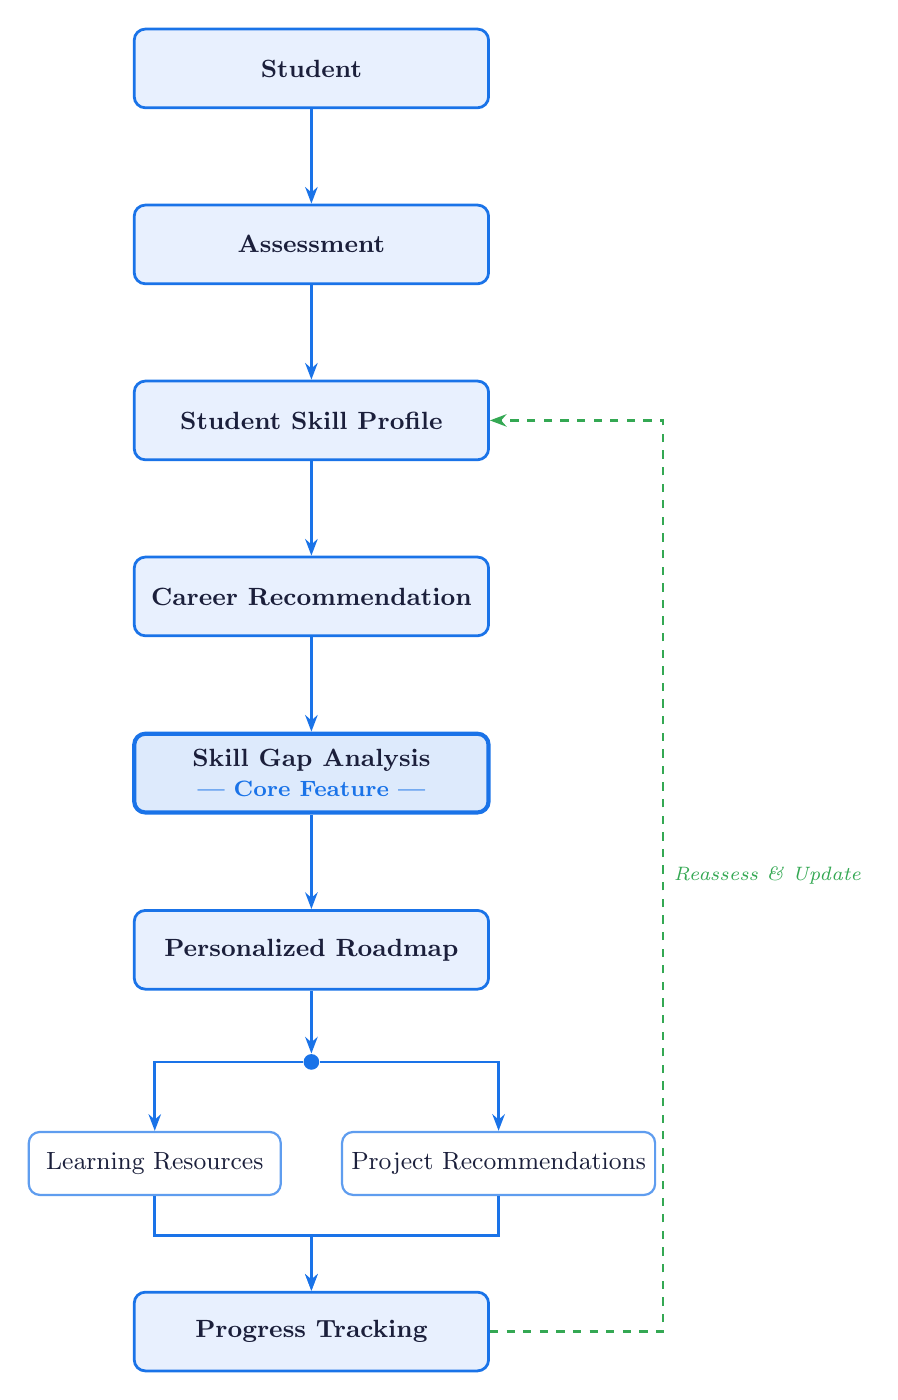
\begin{tikzpicture}[
    node distance=1.2cm,
    box/.style={
      rectangle, rounded corners=4pt, draw=masarblue, line width=1pt,
      fill=masarlight, text=masardark, font=\small\bfseries,
      minimum width=4.5cm, minimum height=1cm, align=center
    },
    smallbox/.style={
      rectangle, rounded corners=4pt, draw=masarblue!70, line width=0.8pt,
      fill=white, text=masardark, font=\small,
      minimum width=3.2cm, minimum height=0.8cm, align=center
    },
    arr/.style={-{Stealth[length=6pt]}, masarblue, line width=1pt},
    splitdot/.style={circle, fill=masarblue, inner sep=2pt},
  ]

  \node[box] (student) {Student};
  \node[box, below=of student] (assess) {Assessment};
  \node[box, below=of assess] (profile) {Student Skill Profile};
  \node[box, below=of profile] (career) {Career Recommendation};
  \node[box, below=of career, fill=masarblue!15, draw=masarblue, line width=1.5pt] (gap) {Skill Gap Analysis\\{\footnotesize\textcolor{masarblue}{--- Core Feature ---}}};
  \node[box, below=of gap] (roadmap) {Personalized Roadmap};

  \node[splitdot, below=0.8cm of roadmap] (split) {};

  \node[smallbox, below left=0.8cm and 0.3cm of split] (resources) {Learning Resources};
  \node[smallbox, below right=0.8cm and 0.3cm of split] (projects) {Project Recommendations};

  \node[box, below=2.8cm of split] (progress) {Progress Tracking};

  % Arrows
  \draw[arr] (student) -- (assess);
  \draw[arr] (assess) -- (profile);
  \draw[arr] (profile) -- (career);
  \draw[arr] (career) -- (gap);
  \draw[arr] (gap) -- (roadmap);
  \draw[arr] (roadmap) -- (split);
  \draw[arr] (split) -| (resources);
  \draw[arr] (split) -| (projects);
  \draw[arr] (resources.south) -- ++(0,-0.5) -| (progress.north);
  \draw[arr] (projects.south) -- ++(0,-0.5) -| (progress.north);

  % Feedback loop
  \draw[arr, masargreen, dashed, line width=0.8pt]
    (progress.east) -- ++(2.2,0) |- node[right, pos=0.25, font=\scriptsize\itshape, text=masargreen]{Reassess \& Update} (profile.east);

\end{tikzpicture}
\end{center}

\newpage

% ============================================================================
% SECTION 3: MVP FEATURES (DETAILED)
% ============================================================================
\section{MVP Feature Specification}

% --- 3.1 Student Profile ---------------------------------------------------
\subsection{Student Profile}
\label{sec:mvp-profile}

The student provides the following information to build their profile:

\begin{itemize}[leftmargin=1.5cm]
  \item Academic year / background
  \item Current technical skills (self-assessed proficiency)
  \item Interests and preferences
  \item Previous courses taken
  \item Projects completed
  \item Career preferences and goals
\end{itemize}

\noindent This data feeds directly into the Assessment and Skill Gap Analysis modules.

% --- 3.2 Career Assessment -------------------------------------------------
\subsection{Career Assessment}
\label{sec:mvp-assessment}

A structured assessment covering:

\begin{itemize}[leftmargin=1.5cm]
  \item Technical knowledge depth
  \item Programming and problem-solving ability
  \item Interest areas
  \item Career preferences
\end{itemize}

\noindent The result produces ranked career recommendations:

\begin{center}
\begin{tabular}{@{} r l c @{}}
\toprule
\textbf{Rank} & \textbf{Career Path} & \textbf{Match Score} \\
\midrule
1 & Backend Development      & 84\% \\
2 & AI Engineering           & 76\% \\
3 & Data Engineering         & 69\% \\
\bottomrule
\end{tabular}
\end{center}

\noindent\textit{The recommendation can initially use a \textbf{weighted scoring algorithm}. Sophisticated ML is not required for the MVP.}

% --- 3.3 Career & Skill Database -------------------------------------------
\subsection{Career \& Skill Database}
\label{sec:mvp-database}

The MVP targets \textbf{5--6 career paths}:

\begin{center}
\begin{tabular}{@{} c l @{}}
\toprule
\textbf{\#} & \textbf{Career Path} \\
\midrule
1 & Software / Full-Stack Development \\
2 & Backend Development \\
3 & AI / Machine Learning \\
4 & Data Engineering / Data Science \\
5 & Cybersecurity \\
6 & DevOps / Cloud \\
\bottomrule
\end{tabular}
\end{center}

\noindent Each career has a defined set of skills and their importance levels.

\bigskip
\noindent\textbf{Example --- Backend Developer Skill Requirements:}

\begin{center}
\begin{tabular}{@{} l c @{}}
\toprule
\textbf{Skill} & \textbf{Importance} \\
\midrule
Python   & 90\% \\
SQL      & 85\% \\
APIs     & 85\% \\
Git      & 70\% \\
Docker   & 60\% \\
Testing  & 60\% \\
Cloud    & 40\% \\
\bottomrule
\end{tabular}
\end{center}

% --- 3.4 Skill-Gap Analysis ------------------------------------------------
\subsection{Skill-Gap Analysis --- Core Feature}
\label{sec:mvp-gap}

This is the \textbf{heart of Masar}. The system compares the student's current skill profile against the target career's requirements and classifies each skill.

\bigskip
\noindent\textbf{Example --- Student targeting ``Backend Developer'':}

\begin{center}
\begin{tabular}{@{} l c c l @{}}
\toprule
\textbf{Skill} & \textbf{Student} & \textbf{Target} & \textbf{Status} \\
\midrule
Python  & 80\% & 90\% & \strongmark\ Strong \\
Git     & 90\% & 70\% & \strongmark\ Strong \\
APIs    & 70\% & 85\% & \warnmark\ Needs Improvement \\
SQL     & 55\% & 85\% & \warnmark\ Needs Improvement \\
Docker  & 20\% & 60\% & \gapmark\ High Priority Gap \\
Testing & 35\% & 60\% & \gapmark\ High Priority Gap \\
\bottomrule
\end{tabular}
\end{center}

\noindent The system also explains \textbf{why each gap matters} in the context of the target career.

% --- 3.5 Personalized Roadmap ----------------------------------------------
\subsection{Personalized Roadmap}
\label{sec:mvp-roadmap}

Based on the identified gaps, Masar generates an ordered learning roadmap that respects prerequisites.

\begin{center}
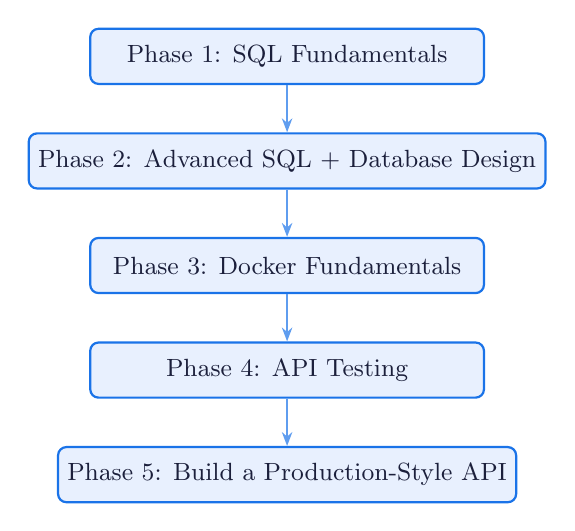
\begin{tikzpicture}[
    node distance=0.6cm,
    phase/.style={
      rectangle, rounded corners=3pt, draw=masarblue, line width=0.8pt,
      fill=masarlight, text=masardark, font=\small,
      minimum width=5cm, minimum height=0.7cm, align=center
    },
    arr/.style={-{Stealth[length=5pt]}, masarblue!70, line width=0.8pt},
  ]
  \node[phase] (p1) {Phase 1: SQL Fundamentals};
  \node[phase, below=of p1] (p2) {Phase 2: Advanced SQL + Database Design};
  \node[phase, below=of p2] (p3) {Phase 3: Docker Fundamentals};
  \node[phase, below=of p3] (p4) {Phase 4: API Testing};
  \node[phase, below=of p4] (p5) {Phase 5: Build a Production-Style API};

  \draw[arr] (p1) -- (p2);
  \draw[arr] (p2) -- (p3);
  \draw[arr] (p3) -- (p4);
  \draw[arr] (p4) -- (p5);
\end{tikzpicture}
\end{center}

\noindent\textit{AI can contribute to roadmap generation, but the underlying skill ordering should remain controlled by the system's prerequisite graph.}

% --- 3.6 Learning Resources ------------------------------------------------
\subsection{Learning Resources}
\label{sec:mvp-resources}

Each roadmap item receives curated, relevant learning resources.

\bigskip
\noindent\textbf{Example --- ``Learn Docker'':}

\begin{center}
\begin{tabular}{@{} l l @{}}
\toprule
\textbf{Attribute} & \textbf{Value} \\
\midrule
Level          & Beginner \\
Resources      & Docker documentation, Introductory course, Practice exercises \\
Estimated Time & 8 hours \\
Prerequisites  & Basic Linux \\
\bottomrule
\end{tabular}
\end{center}

\noindent\textit{For the MVP, maintain a \textbf{curated database of resources} rather than asking an LLM to generate URLs.}

% --- 3.7 Project Recommendations -------------------------------------------
\subsection{Project Recommendations}
\label{sec:mvp-projects}

Masar recommends hands-on projects selected based on the student's skill gaps. This makes Masar more than a course recommender.

\bigskip
\noindent\textbf{Example --- ``Containerized REST API'' Project:}

\begin{center}
\begin{tabular}{@{} l l @{}}
\toprule
\textbf{Attribute} & \textbf{Details} \\
\midrule
Project Title   & Containerized REST API \\
Skills Developed & REST APIs, PostgreSQL, Docker, Testing, Git \\
Basis           & Selected from the student's identified skill gaps \\
\bottomrule
\end{tabular}
\end{center}

% --- 3.8 Progress Tracking -------------------------------------------------
\subsection{Progress Tracking}
\label{sec:mvp-progress}

The student can mark completed items, and the system updates the profile accordingly.

\bigskip
\noindent\textbf{Example:}
\begin{itemize}[leftmargin=1.5cm]
  \item[\strongmark] Completed SQL course
  \item[\strongmark] Completed Docker fundamentals
  \item[\strongmark] Built API project
\end{itemize}

\noindent\textbf{Profile Update:}
\begin{center}
\begin{tabular}{@{} l c c @{}}
\toprule
\textbf{Skill} & \textbf{Before} & \textbf{After} \\
\midrule
Docker & 20\% & 55\% \\
\bottomrule
\end{tabular}
\end{center}

\noindent Masar then updates the roadmap, providing the beginning of the \textbf{adaptive} learning cycle (see the dashed feedback arrow in the system flow diagram, Section~2.1).

\newpage

% ============================================================================
% SECTION 4: AI COMPONENTS IN THE MVP
% ============================================================================
\section{AI Components}

AI is an \textbf{enabling component} of Masar, not the product itself. For the MVP, three focused AI tasks are defined.

% --- 4.1 Job/Resource Skill Extraction --------------------------------------
\subsection{AI Task 1: Job / Resource Skill Extraction}
\label{sec:ai-extraction}

\textbf{Goal:} Extract structured skill requirements from unstructured job postings or resource descriptions using NLP.

\bigskip
\noindent\textbf{Example Input:}
\begin{quote}
\textit{``Looking for a backend developer with Python, PostgreSQL, Docker and REST API experience.''}
\end{quote}

\noindent\textbf{Extracted Output:}

\begin{center}
\begin{tabular}{@{} l @{}}
\toprule
\textbf{Extracted Skill} \\
\midrule
Python \\
PostgreSQL \\
Docker \\
REST APIs \\
\bottomrule
\end{tabular}
\end{center}

% --- 4.2 Semantic Career Matching -------------------------------------------
\subsection{AI Task 2: Semantic Career Matching}
\label{sec:ai-matching}

\textbf{Goal:} Use embeddings to semantically relate skills and career terms beyond exact keyword matching.

\bigskip
\noindent\textbf{Example:}
\begin{center}
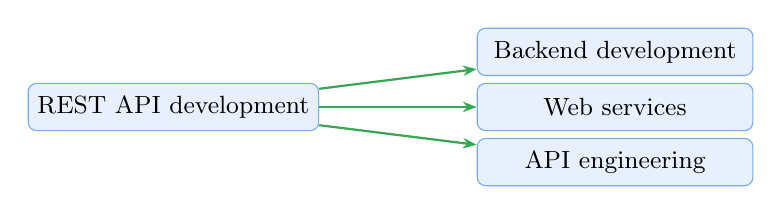
\begin{tikzpicture}[
    node distance=0.3cm and 2cm,
    term/.style={
      rectangle, rounded corners=3pt, draw=masarblue!60, fill=masarlight,
      font=\small, minimum width=3.5cm, minimum height=0.6cm, align=center
    },
    rel/.style={-{Stealth[length=5pt]}, masargreen, line width=0.8pt},
  ]
  \node[term] (input) {REST API development};
  \node[term, right=of input, yshift=0.7cm] (r1) {Backend development};
  \node[term, right=of input] (r2) {Web services};
  \node[term, right=of input, yshift=-0.7cm] (r3) {API engineering};

  \draw[rel] (input) -- (r1);
  \draw[rel] (input) -- (r2);
  \draw[rel] (input) -- (r3);
\end{tikzpicture}
\end{center}

% --- 4.3 AI Mentor ---------------------------------------------------------
\subsection{AI Task 3: AI Mentor}
\label{sec:ai-mentor}

\textbf{Goal:} Provide context-aware guidance using the student's profile and roadmap.

\bigskip
\noindent\textbf{Example Interaction:}

\begin{quote}
\textbf{Student:} ``Why should I learn Docker?''

\textbf{Masar:} \textit{``Docker is currently one of your largest skill gaps for backend development. It's included in your roadmap because it appears frequently in the requirements of the backend roles you're targeting.''}
\end{quote}

\noindent This is an achievable LLM-based feature that grounds responses in the student's actual data.

\newpage

% ============================================================================
% SECTION 5: FEATURE CLASSIFICATION & PRIORITY
% ============================================================================
\section{Feature Classification \& Priority Matrix}

Features are classified into four tiers to define what constitutes project completion at each stage.

\subsection{Priority Tiers}

\begin{description}[style=nextline, leftmargin=2cm]
  \item[\textcolor{masarred}{\textbf{MVP -- Core}}]
    Features without which the product cannot demonstrate its central value proposition. The project \textbf{cannot be considered functional} without these.

  \item[\textcolor{masarorange}{\textbf{MVP}}]
    Features required for a complete MVP demonstration. The project is \textbf{considered done at MVP level} with these.

  \item[\textcolor{masarblue}{\textbf{Should Have}}]
    Features that significantly enhance the product and should be targeted after MVP completion. Having these moves the project from ``functional'' to ``polished.''

  \item[\textcolor{masargray}{\textbf{Nice to Have / Later}}]
    Features that are out of scope for the core project but represent natural extensions.
\end{description}

\subsection{Complete Feature Priority Matrix}

\begin{center}
\renewcommand{\arraystretch}{1.3}
\begin{tabularx}{\textwidth}{@{} X c @{}}
\toprule
\textbf{Feature} & \textbf{Priority Tier} \\
\midrule
\multicolumn{2}{@{}l}{\textbf{\textcolor{masardark}{--- The product is NOT demonstrable without these ---}}} \\
\addlinespace[3pt]
Skill-Gap Analysis (core engine)
  & \textcolor{masarred}{\textbf{MVP -- Core}} \\
Personalized Roadmap Generation
  & \textcolor{masarred}{\textbf{MVP -- Core}} \\

\addlinespace[6pt]
\multicolumn{2}{@{}l}{\textbf{\textcolor{masardark}{--- The MVP is complete with these ---}}} \\
\addlinespace[3pt]
Student Profile
  & \textcolor{masarorange}{\textbf{MVP}} \\
Career Assessment
  & \textcolor{masarorange}{\textbf{MVP}} \\
Career Recommendation
  & \textcolor{masarorange}{\textbf{MVP}} \\
Career \& Skill Database
  & \textcolor{masarorange}{\textbf{MVP}} \\
Learning Resources (curated)
  & \textcolor{masarorange}{\textbf{MVP}} \\
Project Recommendations
  & \textcolor{masarorange}{\textbf{MVP}} \\
Progress Tracking
  & \textcolor{masarorange}{\textbf{MVP}} \\

\addlinespace[6pt]
\multicolumn{2}{@{}l}{\textbf{\textcolor{masardark}{--- Should target after MVP; enhances quality significantly ---}}} \\
\addlinespace[3pt]
Basic AI Mentor (LLM-based)
  & \textcolor{masarblue}{\textbf{Should Have}} \\
Job-Skill NLP Extraction
  & \textcolor{masarblue}{\textbf{Should Have}} \\
Semantic Career Matching (Embeddings)
  & \textcolor{masarblue}{\textbf{Should Have}} \\

\addlinespace[6pt]
\multicolumn{2}{@{}l}{\textbf{\textcolor{masardark}{--- Out of MVP scope; future enhancements ---}}} \\
\addlinespace[3pt]
Job Matching
  & \textcolor{masargray}{\textbf{Later}} \\
Resume Builder
  & \textcolor{masargray}{\textbf{Later}} \\
ATS Optimization
  & \textcolor{masargray}{\textbf{Later}} \\
Interview Simulator
  & \textcolor{masargray}{\textbf{Later}} \\
GitHub Profile Analysis
  & \textcolor{masargray}{\textbf{Later}} \\
Calendar Integration
  & \textcolor{masargray}{\textbf{Later}} \\
Flutter Mobile App
  & \textcolor{masargray}{\textbf{Later}} \\
Large-Scale Job Scraping
  & \textcolor{masargray}{\textbf{Later}} \\
\bottomrule
\end{tabularx}
\end{center}

\subsection{Completion Criteria Summary}

\begin{center}
\renewcommand{\arraystretch}{1.4}
\begin{tabularx}{\textwidth}{@{} l X @{}}
\toprule
\textbf{Milestone} & \textbf{Definition of Done} \\
\midrule
\textbf{MVP -- Core} &
  A student can input their skills, select a target career, see the gap analysis, and receive an ordered roadmap. The fundamental value loop is demonstrable. \\

\textbf{MVP -- Complete} &
  All MVP-tier features are functional: profile creation, assessment, career recommendation, curated resources, project suggestions, and progress tracking with profile updates. \\

\textbf{Enhanced Product} &
  Should-Have AI features (mentor, NLP extraction, semantic matching) are integrated, making the system intelligent beyond rule-based logic. \\

\textbf{Full Product Vision} &
  Later-tier features are added, transforming Masar into a comprehensive career development platform with job matching, resume tools, and mobile access. \\
\bottomrule
\end{tabularx}
\end{center}

\newpage

% ============================================================================
% SECTION 6: FEATURE DETAILS — SHOULD HAVE
% ============================================================================
\section{Should-Have Features (Post-MVP)}

These features elevate the project from a functional prototype to an intelligent system. They should be the primary targets after the MVP is stable.

\subsection{Basic AI Mentor}
An LLM-powered conversational assistant that answers learning and career questions using the student's profile, roadmap, and skill-gap data as context. Responses are grounded in the student's actual situation rather than generic advice.

\subsection{Job-Skill NLP Extraction}
An NLP pipeline that processes job postings and extracts structured skill requirements. This keeps the skill database current with industry trends and reduces manual curation effort.

\subsection{Semantic Career Matching}
Using embedding models to match student skills to careers beyond keyword overlap. For example, recognizing that ``REST API development'' experience is relevant to ``Backend Development,'' ``Web Services,'' and ``API Engineering'' roles.

\newpage

% ============================================================================
% SECTION 7: LATER / NICE-TO-HAVE FEATURES
% ============================================================================
\section{Nice-to-Have Features (Future Vision)}

These features are explicitly \textbf{out of MVP scope}. They represent natural product extensions for future development phases.

\begin{center}
\renewcommand{\arraystretch}{1.3}
\begin{tabularx}{\textwidth}{@{} l X @{}}
\toprule
\textbf{Feature} & \textbf{Description} \\
\midrule
Job Matching &
  Match students directly with real job postings based on their profile and skill level. \\

Resume Builder &
  Generate ATS-friendly resumes tailored to specific target roles. \\

ATS Optimization &
  Analyze and optimize resumes for applicant tracking systems used by employers. \\

Interview Simulator &
  Practice technical and behavioral interviews with AI-generated questions and feedback. \\

GitHub Analysis &
  Analyze a student's GitHub repositories to automatically assess demonstrated skills and project complexity. \\

Calendar Integration &
  Schedule learning activities and set milestone reminders within the student's calendar. \\

Flutter Mobile App &
  A cross-platform mobile application for on-the-go access to roadmaps and progress tracking. \\

Large-Scale Job Scraping &
  Automated collection of job postings to keep the skill database aligned with real-time market demand. \textit{Should not be made a core dependency.} \\
\bottomrule
\end{tabularx}
\end{center}

\vspace{1cm}

\begin{center}

\begin{tikzpicture}
  \draw[masarblue, line width=1.5pt] (-4,0) -- (4,0);
  \node[above=0.3cm, font=\small\itshape, text=masargray] at (0,0) {End of Document};
\end{tikzpicture}
\end{center}

\end{document}
